Model grafowy dla Neo4j stanowi najistotniejsze odwzorowanie domeny problemu
spośród trzech analizowanych podejść, ponieważ relacje między encjami zostały
podniesione do rangi obiektów pierwszej klasy. Schemat składa się z dziewięciu
typów węzłów oraz dwunastu typów relacji, ze szczególnym uwzględnieniem
właściwości przypisywanych krawędziom. Strukturę przedstawiono na
rysunku~\ref{fig:schema_neo4j}.

\begin{figure}[H]
    \centering
    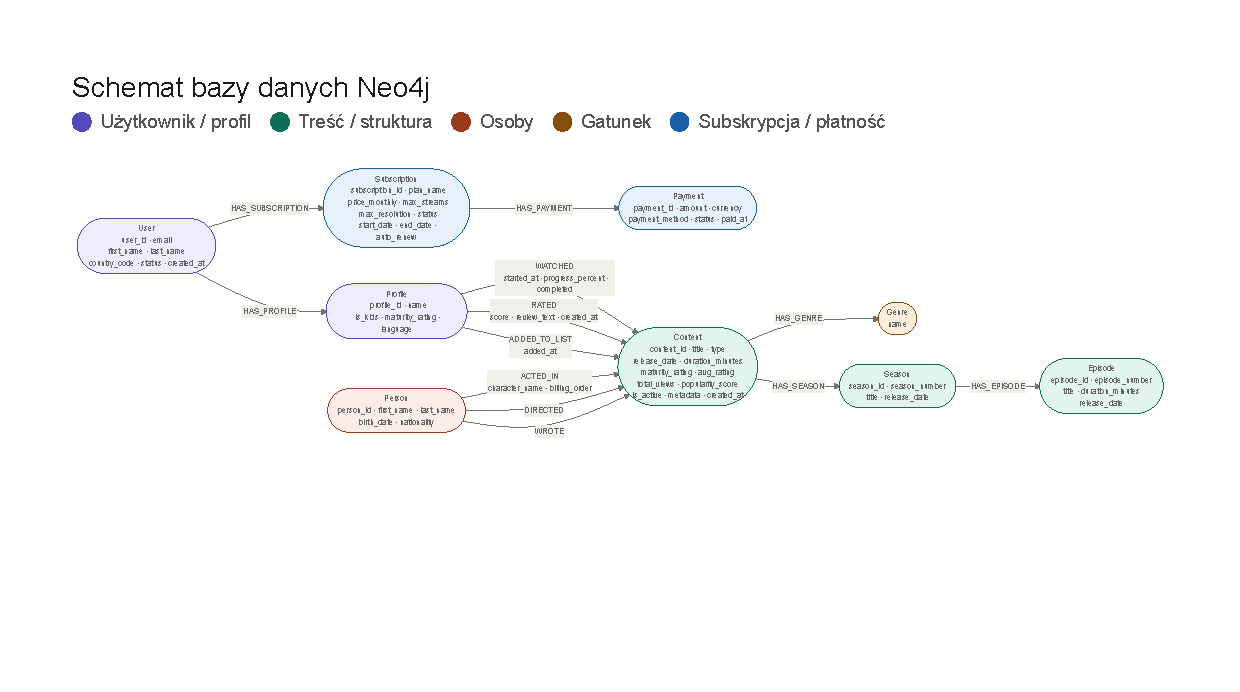
\includegraphics[width=1.0\textwidth]{charts/SchematBazy_neo4j_cropped.pdf}
    \caption{Schemat grafowy dla Neo4j}
    \label{fig:schema_neo4j}
\end{figure}

Domena użytkownika reprezentowana jest przez węzły \texttt{User} oraz
\texttt{Profile}, połączone relacją \texttt{HAS\_PROFILE}. Subskrypcja
została wymodelowana jako odrębny węzeł \texttt{Subscription} powiązany
z użytkownikiem relacją \texttt{HAS\_SUBSCRIPTION}, natomiast historia
płatności obejmuje węzły \texttt{Payment} podpięte do odpowiadających im
subskrypcji relacją \texttt{HAS\_PAYMENT}. Wybór reprezentacji subskrypcji
oraz płatności jako pełnoprawnych węzłów, a nie właściwości użytkownika,
umożliwia efektywne realizowanie zapytań analitycznych, takich jak
identyfikacja użytkowników z aktywną subskrypcją typu \textit{Premium}
lub agregacja przychodów według metody płatności w ustalonym oknie czasowym.

Domena katalogu treści jest zorganizowana wokół centralnego węzła
\texttt{Content}, łączącego się z hierarchią węzłów \texttt{Season} oraz
\texttt{Episode} poprzez relacje \texttt{HAS\_SEASON} oraz
\texttt{HAS\_EPISODE}. Gatunki zostały wymodelowane jako odrębne węzły
\texttt{Genre} powiązane z treścią relacją \texttt{HAS\_GENRE} -- struktura
ta umożliwia efektywne wyszukiwanie treści powiązanych wspólnym gatunkiem
oraz analizę popularności poszczególnych kategorii bez konieczności
skanowania pełnego katalogu. Osoby uczestniczące w produkcji reprezentowane
są przez węzły \texttt{Person}, połączone z węzłami \texttt{Content} przez
trzy odrębne typy relacji: \texttt{ACTED\_IN}, \texttt{DIRECTED} oraz
\texttt{WROTE}. Rozdzielenie ról na osobne typy relacji, zamiast zakodowania
ich jako właściwości pojedynczej krawędzi, umożliwia precyzyjne kierowanie
zapytań oraz wykorzystanie wbudowanej optymalizacji silnika dla konkretnego
typu krawędzi.

Domena aktywności użytkownika została w całości odwzorowana przez relacje
łączące węzły \texttt{Profile} z węzłami \texttt{Content}. Relacja
\texttt{WATCHED} reprezentuje sesje odtwarzania i posiada właściwości
\texttt{started\_at}, \texttt{progress\_percent} oraz \texttt{completed},
przeniesione z tabeli \texttt{watch\_history} modelu relacyjnego. Relacja
\texttt{RATED} przechowuje oceny treści wraz z ich wartością liczbową
(\texttt{score}), opcjonalnym tekstem recenzji (\texttt{review\_text}) oraz
znacznikiem czasu (\texttt{created\_at}). Lista treści dodanych przez
profil reprezentowana jest przez relację \texttt{ADDED\_TO\_LIST}
z właściwością \texttt{added\_at}. Reprezentacja tych encji jako relacji
zamiast węzłów wynika z faktu, że nie posiadają one istotnej tożsamości
poza powiązaniem dwóch obiektów -- profilu oraz treści.

Analogicznie do relacji aktywności, relacja \texttt{ACTED\_IN} przechowuje
właściwości \texttt{character\_name} oraz \texttt{billing\_order}, charakteryzujące
konkretną rolę aktorską, a nie samą osobę. Pozwala to na zwięzłe wyrażanie
zapytań typu „znajdź wszystkich aktorów grających pierwsze role w filmach
nominowanych do określonej nagrody" w pojedynczym wzorcu Cypher,
unikającym wielokrotnych operacji złączenia.

Identyfikatory zewnętrzne zostały zachowane jako właściwości węzłów
(\texttt{user\_id}, \texttt{content\_id} i analogiczne), niezależnie od
wewnętrznych identyfikatorów silnika Neo4j, co umożliwia bezpośrednią
porównywalność danych pomiędzy modelami w trakcie testów wydajnościowych.
Indeksy zostały założone na właściwościach wykorzystywanych w warunkach
filtrujących typowych zapytań -- \texttt{User.email}, \texttt{Content.title},
\texttt{Content.type} oraz \texttt{Person.last\_name} -- co umożliwia silnikowi
zlokalizowanie punktu startowego trawersu grafu w czasie logarytmicznym.
